\documentclass[12pt]{extarticle}
\usepackage{phys440}

\title{PHYS440 - Project: HHL Algorithm}
\author{John Hurst}
\date{June 2024}

\begin{document}
\maketitle

\tableofcontents

\newpage

%%%%%%%%%%%%%%%%%%%%%%%%%%%%%%%%%%%%%%%%%%%%%%%%%%%%%%%%%%%%%%%%%%%%%%%%%%%%%%%%%%%%%%%%%%%%%%%%%%%%
\section{Introduction}

The Harrow-Hassidim-Lloyd (HHL) algorithm for solving linear systems\cite{hhl2009} is
the first of the quantum linear system algorithms (QLSAs),
and one of the first algorithms to promise a quantum speedup for a variety of real-world problems.
The walk-through in \cite{zaman2023step} shows the mathematics for each step and provides background on the relevant quantum computing concepts.
The paper gives a numerical example to illustrate the steps, and provides MATLAB and Qiskit code for the example.

For my PHYS440 project I studied the walkthrough to understand the HHL algorithm in some detail,
and supplemented this by reading several other introductory sources such as \cite{baaquie2023} and \cite{hidary2021}.

I ported the MATLAB sample code to two different Mathematica implementations.
The first implementation is a direct port of the matrix formulation of the circuit from MATLAB.
The second implementation uses the Wolfram Quantum Framework to implement the example using the QuantumCircuitOperator feature.

The paper's example uses a 2x2 matrix, and only two clock qubits, which does not sufficiently illustrate some features of the algorithm.
I created my own example with a 4x4 matrix and three clock qubits, to study these features in more detail.

I verified my example in Mathematica, and in a Qiskit program run on the IBM Quantum simulator.
I then created a more general Qiskit program to explore the behaviour and limits of the algorithm with larger matrices and more clock qubits.

I followed up with some more reading on the limits and applicability of HHL, starting from Aaronson's well-known paper \cite{aaronson2015read}.

The remainder of this report is in several parts.
\begin{itemize}
\item Part \ref{sec:implementation} discusses implementation details of the more general 4x4 numerical example, in particular the handling of the ancilla rotation.
\item Part \ref{sec:generalization} describes some experiments with larger systems and more clock qubits.
\item Part \ref{sec:developments} reviews literature on developments of the HHL algorithm with regard to applications to real word problems.
\end{itemize}

\section{Implementation Notes}\label{sec:implementation}



This report will not repeat all the details from \cite{zaman2023step}.
I will focus instead on what I found by generalising the example to a larger matrix and number of clock qubits.

\subsection{Example 4x4 problem}

For the sample problem, I constructed a 4x4 Hermitian matrix with ``friendly'' eigenvalues in ratio 1:2:3:4,
so that they could be represented exactly using 3 clock qubits.

I defined the matrix like this:
\begin{equation}\label{eq:matrixa4}
A = H_4 \begin{pmatrix}
    \frac{1}{3} & 0 & 0 & 0 \\
    0 & \frac{2}{3} & 0 & 0 \\
    0 & 0 & 1 & 0 \\
    0 & 0 & 0 & \frac{4}{3}
\end{pmatrix} H_4^{\dagger}
= \begin{pmatrix}
    \frac{5}{6} & -\frac{1}{3} & 0 & -\frac{1}{6} \\
    -\frac{1}{3} & \frac{5}{6} & -\frac{1}{6} & 0 \\
    0 & -\frac{1}{6} & \frac{5}{6} & -\frac{1}{3} \\
    -\frac{1}{6} & 0 & -\frac{1}{3} & \frac{5}{6}
\end{pmatrix}
\end{equation}
where $H_4$ is a 4x4 Hadamard matrix.
(There are different possible 4x4 Hadamard matrices, and a common choice is $H_4=H_2\otimes H_2$, but I used Mathematica's \texttt{HadamardMatrix[4]}, which is different.)

For $b$ I used
\begin{equation}\label{eq:vectorb4}
b = \begin{pmatrix} 1 \\ 2 \\ 3 \\ 2 \end{pmatrix}
\end{equation}

The solution is given by
\begin{equation}\label{eq:solutionx4}
A^{-1}b = \frac{1}{4}\begin{pmatrix} 19 \\ 23 \\ 29 \\ 25 \end{pmatrix}
\end{equation}
In the HHL algorithm with solution is scaled because it is read from the relative frequencies of different measurements.
For the purpose of checking the algorithm we'll use a scaled solution such that the elements sum to 1:
\begin{equation}\label{eq:solutionx4num}
x = \begin{pmatrix} 0.1979 \\ 0.2396 \\ 0.3021 \\ 0.2604 \end{pmatrix}
\end{equation}

\subsection{Circuit details}

My HHL circuit for a 4x4 matrix and three clock qubits is shown in Figures \ref{fig:circuit1}-\ref{fig:circuit3}.
The first register, labelled $b$, with two qubits, begins with the input state, and carries the result $x$ at the end.
The second register, labelled $q$, with three qubits, is the clock register.
The third register, labelled $a$, with one qubit, is the ancilla register.

Figure \ref{fig:circuit1} shows the state preparation and QPE.
Because the goal of my implementation is to understand the algorithm,
not to provide a practical implementation, I have provided the input state directly in Mathematica using the \texttt{QuantumTensorProduct[]} function:
\begin{lstlisting}[language=Mathematica]
psi1 =
    QuantumTensorProduct[
        Join[{QuantumState[Normalize[b]]},
              ConstantArray[QuantumState[{1, 0}], n + 1]]]
\end{lstlisting}
\begin{figure}[h]
\centering
$\begin{array}{c}
\Qcircuit @C=.5em @R=.8em {
\lstick{a}   & \qw & \qw      & \qw       & \qw & \qw & \qw & \qw & \qw & \qw & \qw & \qw & \qw & \qw & \qw \\
& & & & & & & \mbox{IQFT} & & & & & & & \\
\lstick{q_0} & \qw & \gate{H} & \ctrl{3} & \qw & \qw & \qswap & \gate{H} & \ctrl{1} & \qw & \ctrl{2} & \qw & \qw & \qw & \qw \\
\lstick{q_1} & \qw & \gate{H} & \qw & \ctrl{2} & \qw & \qw & \qw & \gate{R_{-1/2}} & \gate{H} & \qw & \ctrl{1} & \qw & \qw & \qw \\
\lstick{q_2} & \qw & \gate{H} & \qw & \qw & \ctrl{1} & \qswap \qwx[-2] & \qw & \qw & \qw & \gate{R_{-1/4}} & \gate{R_{-1/2}} & \gate{H} & \qw & \qw \\
\lstick{b_0} & \multigate{1}{\text{prepare } b} & \qw & \multigate{1}{U} & \multigate{1}{U^2} & \multigate{1}{U^4} & \qw & \qw & \qw & \qw & \qw & \qw & \qw & \qw & \qw \\
\lstick{b_1} & \ghost{\text{prepare } b} & \qw & \ghost{U} & \ghost{U^2} & \ghost{U^4} & \qw & \qw & \qw & \qw & \qw & \qw & \qw & \qw & \qw
\gategroup{2}{7}{5}{13}{1.4em}{--}
}
\end{array}$
\caption{State preparation and QPE}
\label{fig:circuit1}
\end{figure}
In real world applications, state preparation is a nontrivial problem, as discussed in \cite{aaronson2015read} and \cite{hhl2009}.

This part of the circuit is conceptually the same as in \cite{zaman2023step},
but because there are four values in the input $b$ and four unknowns in $x$, the unitary operation in the QPE has two target qubits instead of one.
Also, because there are three clock qubits, in QPE we apply $U$, $U^2$ and $U^4$, and the IQFT subcomponent is extended to three qubits.

Figure \ref{fig:circuit2} shows the ancilla rotation.
\begin{figure}[h]
\centering
$\begin{array}{c}
\Qcircuit @C=.5em @R=.8em {
\lstick{a}   & \qw & \gate{RY(\theta_1=2\inv{\sin}\frac{1}{4})} & \gate{RY(\theta_2=2\inv{\sin}\frac{1}{3})} & \gate{RY(\theta_3=\frac{\pi}{3})} & \gate{RY(\theta_4=\pi)} & \qw \\
\lstick{q_0} & \qw & \ctrlo{-1} & \ctrl{-1}  & \ctrlo{-1} & \ctrl{-1}  & \qw \\
\lstick{q_1} & \qw & \ctrlo{-2} & \ctrl{-2}  & \ctrl{-2}  & \ctrlo{-2} & \qw \\
\lstick{q_2} & \qw & \ctrl{-3}  & \ctrlo{-3} & \ctrlo{-3} & \ctrlo{-3} & \qw \\
% \lstick{b_0} & \qw & \qw & \qw & \qw & \qw & \qw \\
% \lstick{b_1} & \qw & \qw & \qw & \qw & \qw & \qw \\
}
\end{array}$
\caption{Ancilla rotation}
\label{fig:circuit2}
\end{figure}

This part of the circuit is the most interesting part of the project.

As discussed in class, I was confused about the number of rotations on the ancilla qubit.
In \cite{zaman2023step} there are two rotations on the ancilla qubit, using angles $\theta_1$ and $\theta_2$, and controlled by the two clock qubits.
The angles $\theta_1$ and $\theta_2$ are calculated from the eigenvalues of the matrix $A$.
So it was unclear to me whether there should be a distinct rotation were per eigenvalue, or per clock qubit.
It seemed to me from the construction of the circuit that it must be a rotation per clock qubit.
And also, in real-world applications we might have billions of unknowns and eigenvalues, but we will always have a fairly limited number of clock qubits, determined by the precision desired.
So it seemed to me that it would not be practical to consider rotations per eigenvalue.

It turns out that my thinking was not correct.
The rotations on the ancilla qubit achieve the inversion of the eigenvalues,
and so to get a solution with perfect accuracy it is necessary to have a rotation per eigenvalue.
However, in real world implementations, it's unlikely this would actually be done for large numbers of input qubits.
By being selective and careful about the rotations, an approximate solution satisfies the accuracy bounds in \cite{hhl2009}.
A recent paper, \cite{morgan2024enhanced}, discusses filtering rotations ``by relevance'' to maintain circuit depth advantages.

In the circuit in Figure \ref{fig:circuit2}, I have implemented four rotations with angles $\theta_1$, $\theta_2$, $\theta_3$ and $\theta_4$,
which correspond precisely to the eigenvalues $\lambda_1$, $\lambda_2$, $\lambda_3$ and $\lambda_4$ of the matrix $A$.
They are controlled by the clock qubits according to the binary representation of the eigenvalue phases on the clock qubits.
So for example, the first eigenvalue is $\lambda_1=\frac{4}{3}$.
In the Hamiltonian $e^{i\Lambda t}$ this eigenvalue has corresponding value $e^{i\lambda_1t}=e^{i\frac{4}{3}\times\frac{3\pi}{4}}=e^{2\pi i \frac{1}{2}}$.
Therefore the phase for this eigenvalue is $\phi_1=\frac{1}{2}$, which in binary is 0.100b.
Therefore the rotation for this eigenvalue should occur when qubit $q_2$ is set and qubits $q_1$ and $q_0$ are not set.
The rotation angle is obtained via the formula from \cite{zaman2023step}: $\theta_1=2\inv{\sin}\bar{\lambda}_1$,
where $\bar{\lambda}_1$ is the eigenvalue scaled by a factor that makes all the eigenvalues integers:
\[
\bar{\lambda_j}=\frac{2^n\lambda_jt}{2\pi}
\]
In this way we obtain the phases, controlling qubits, and rotation angles for all the eigenvalues, shown in the table below:
\begin{center}
\begin{tabular}{|c|c|c|c|c|}
\hline
Eigenvalue & $e^{i\lambda t}=e^{2\pi i\phi}$ & Phase & Qubits & Angle \\
\hline
$\lambda_1=\frac{4}{3}$ & $e^{i\lambda_1t}=e^{i \frac{4}{3} \times \frac{3\pi}{4}}=e^{2\pi i \frac{1}{2}}$ & $\phi_1=\frac{1}{2}=$0.100b & $q_2\overline{q_1}\overline{q_0}$ & $\theta_1=2\inv{\sin}\frac{1}{4}$ \\
$\lambda_2=1$           & $e^{i\lambda_2t}=e^{i 1 \times \frac{3\pi}{4}}=e^{2\pi i \frac{3}{8}}$   & $\phi_2=\frac{3}{8}=$0.011b & $\overline{q_2}q_1q_0$ & $\theta_2=2\inv{\sin}\frac{1}{3}$ \\
$\lambda_3=\frac{2}{3}$ & $e^{i\lambda_3t}=e^{i \frac{2}{3} \times \frac{3\pi}{4}}=e^{2\pi i \frac{1}{4}}$ & $\phi_3=\frac{1}{4}=$0.010b & $\overline{q_2}q_1\overline{q_0}$ & $\theta_3=2=2\inv{\sin}\frac{1}{2}=\frac{\pi}{3}$ \\
$\lambda_4=\frac{1}{3}$ & $e^{i\lambda_4t}=e^{i \frac{1}{3} \times \frac{3\pi}{4}}=e^{2\pi i \frac{1}{8}}$ & $\phi_4=\frac{1}{8}=$0.001b & $\overline{q_2}\overline{q_1}q_0$ & $\theta_4=2=2\inv{\sin}\frac{1}{1}=\pi$ \\
\hline
\end{tabular}
\end{center}
The controlling qubits and rotation angles correspond to the circuit portion in Figure \ref{fig:circuit2}.
% TODO: How might this have been shown more clearly in zaman2023step?

Figure \ref{fig:circuit3} shows the reverse QPE and measurement.
As in \cite{zaman2023step}, if the ancilla qubit is measured in state $\ket{1}$,
then the $b$ register holds the correct $x$ result.
If the ancilla qubit is measured in state $\ket{0}$, the result is discarded and the circuit must be run again.
\begin{figure}[h]
\centering
$\begin{array}{c}
\Qcircuit @C=.4em @R=.7em {
    \lstick{a}   & \qw & \qw & \qw & \qw & \qw & \qw & \qw & \qw & \qw & \qw & \qw & \qw & \meter \\
    & & & \mbox{QFT} & & & & & & & & & & & & \\
    \lstick{q_2} & \qw & \qw & \qw & \ctrl{2} & \qw & \ctrl{1} & \gate{H} & \qswap & \qw & \qw & \ctrl{3} & \gate{H} & \qw \\
    \lstick{q_1} & \qw & \qw & \ctrl{1} & \qw & \gate{H} & \gate{R_{1/2}} & \qw & \qw & \qw & \ctrl{2} & \qw & \gate{H} & \qw \\
    \lstick{q_0} & \qw & \gate{H} & \gate{R_{1/2}} & \gate{R_{1/4}} & \qw & \qw & \qw & \qswap \qwx[-2] & \ctrl{1} & \qw & \qw & \gate{H} & \qw \\
\lstick{b_0} & \qw & \qw & \qw & \qw & \qw & \qw & \qw & \qw & \multigate{1}{U^{-4}} & \multigate{1}{U^{-2}} & \multigate{1}{U^{-1}} & \qw & \meter \\
\lstick{b_1} & \qw & \qw & \qw & \qw & \qw & \qw & \qw & \qw & \ghost{U^{-4}} & \ghost{U^{-2}} & \ghost{U^{-1}} & \qw & \meter
\gategroup{2}{3}{5}{8}{1.4em}{--}
}
\end{array}$
\caption{Inverse QPE and measurement}
\label{fig:circuit3}
\end{figure}

% \begin{figure}[H]
% \centering
% 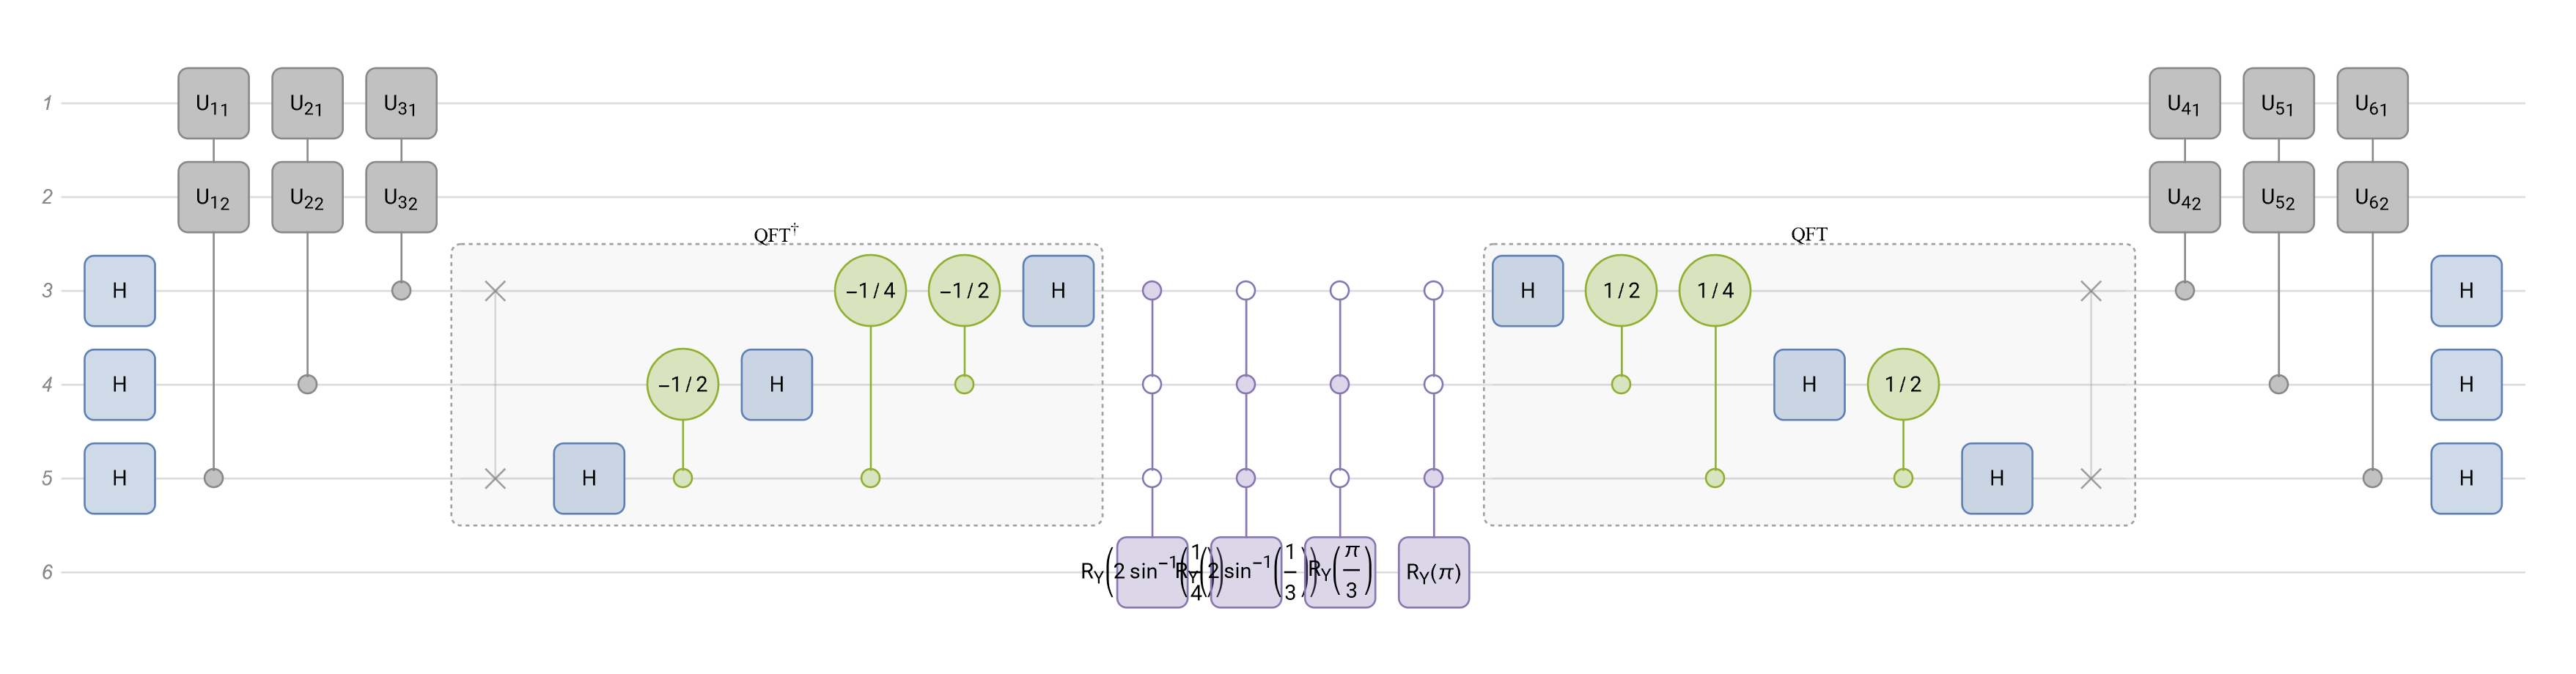
\includegraphics[width=0.80\textwidth]{images/project_hhl_4x4_mathematica.png}
% \caption{Mathematica circuit for 4x4 problem}
% \label{fig:hhl_4x4_mathematica}
% \end{figure}

\subsection{Qiskit circuit implementation}

I wrote a Qiskit program to construct the circuit for the 4x4 problem and run it on the IBM Quantum simulator.
A sample run looks like this:

\begin{lstlisting}[language=Bash]
bin/project_hhl_4x4_qiskit.py --shots=10000 --filename=project_hhl_4x4.png
000000  434
000001  1345    0.1476  0.1944
010000  1
010001  2053    0.2252  0.2402
100000  450
100001  3274    0.3592  0.3033
110001  2443    0.2680  0.2620
Prob(ancilla |0>) = 0.9115
\end{lstlisting}

The first part of the output is a table in four columns:
\begin{itemize}
\item The measurement bits: $b_1$, $b_0$, $q_2$, $q_1$, $q_0$, $a$.
\item The number of times that measurement was observed (the count).
\item The frequency of that measurement: count/total.
\item The square root of the frequency, corresponding to the estimate for the corresponding $x$.
\end{itemize}

Measurements with the ancilla bit (the least significant, or rightmost bit in the output) having value 1 are counted in the result,
and measurements with the ancilla bit having value 0 are discarded.

Following this table is the frequency that the ancilla bit was measured in state $\ket{0}$ (having value 1), in this case 0.9115,
indicating a good effectiveness for the algorithm with these data.

The output from this run is shown more clearly in table \ref{tab:results4x4}, along with the actual $x$ values for comparison.
We can see from the results that with 10,000 shots, we have got pretty good estimates for $x$.

\begin{table}[h]
\begin{center}
\begin{tabular}{|c|r|r|r|r|}
\hline
Measurement & Count & Frequency & $x$ estimate & $x$ actual \\
\hline
000000 &  434 & & & \\
000001 & 1345 & 0.1476 & 0.1944 & 0.1979 \\
010000 &    1 & & & \\
010001 & 2053 & 0.2252 & 0.2402 & 0.2396 \\
100000 &  450 & & & \\
100001 & 3274 & 0.3592 & 0.3033 & 0.3021 \\
110001 & 2443 & 0.2680 & 0.2620 & 0.2604 \\
\hline
\end{tabular}
\caption{Results for 4x4 system}
\label{tab:results4x4}
\end{center}
\end{table}

Figure \ref{fig:hhl_4x4_qiskit} shows the Qiskit circuit for the 4x4 problem.
\begin{figure}[H]
\centering
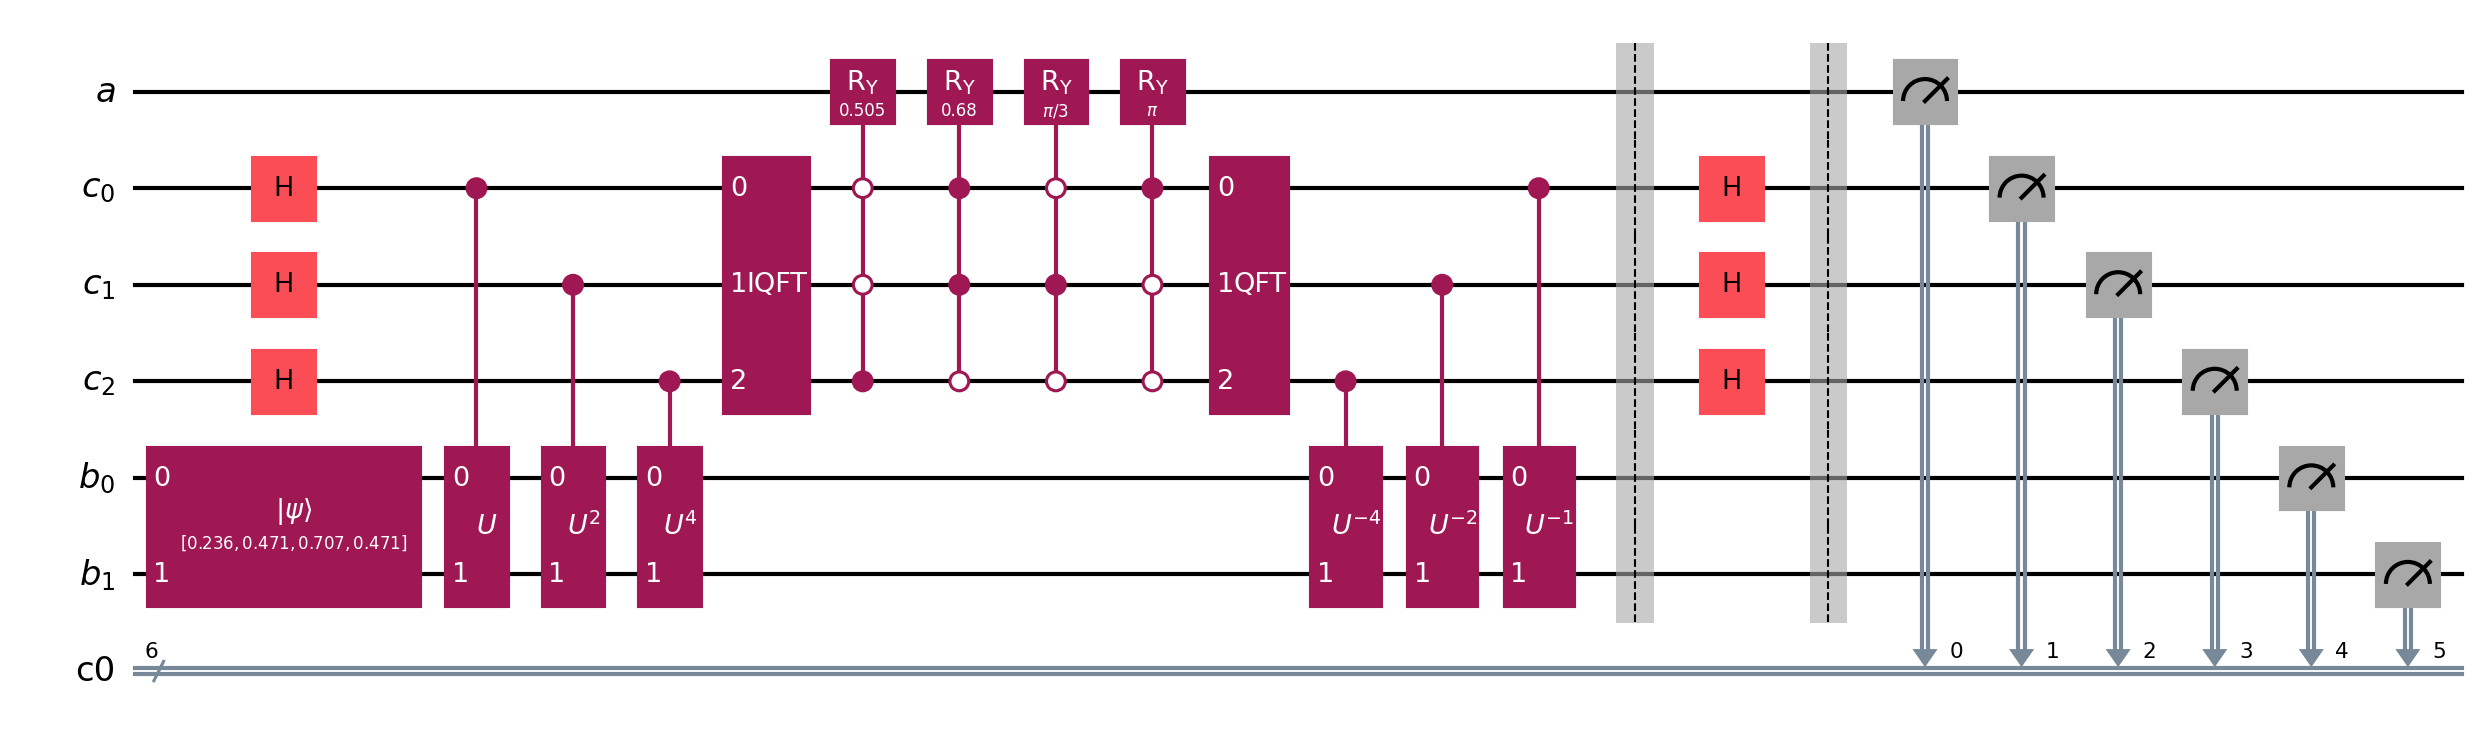
\includegraphics[width=0.80\textwidth]{images/project_hhl_4x4.png}
\caption{Qiskit circuit for 4x4 problem}
\label{fig:hhl_4x4_qiskit}
\end{figure}

\section{Generalization}\label{sec:generalization}

I created a more general Qiskit program to explore the behaviour and limits of the algorithm with larger matrices and more clock qubits.
I also created an 8x8 Hermitian matrix using a similar procedure to above.
This Qiskit program prints the actual $x$ solution values (scaled appropriately), as well as the estimates, to make comparison easier.

For the 8x8 example I ran the program as follows:
\begin{lstlisting}[language=Bash]
bin/project_hhl_qiskit.py --shots=1000000 --clockqubits=6 \
    data/project_hhl/Ahalf_8x8.csv data/project_hhl/b_8x8.csv
\end{lstlisting}

The output is shown in table \ref{tab:results8x8}.

\begin{table}[h]
\begin{center}
\begin{tabular}{|c|r|r|r|r|}
\hline
Measurement & Count & Frequency & $x$ estimate & $x$ actual \\
\hline
0000000000  &  11019 & & & \\
0000000001  &     26 & 0.0000 & 0.0091 & 0.0091 \\
0010000000  &  77671 & & & \\
0010000001  &    609 & 0.0006 & 0.0440 & 0.0435 \\
0100000000  &  80853 & & & \\
0100000001  &  10871 & 0.0109 & 0.1859 & 0.1858 \\
0110000000  &  12558 & & & \\
0110000001  &    451 & 0.0005 & 0.0379 & 0.0377 \\
1000000000  & 230535 & & & \\
1000000001  &   4079 & 0.0041 & 0.1139 & 0.1141 \\
1010000000  &  50226 & & & \\
1010000001  &    370 & 0.0004 & 0.0343 & 0.0329 \\
1100000000  & 110700 & & & \\
1100000001  &   6789 & 0.0068 & 0.1469 & 0.1476 \\
1110000000  & 345591 & & & \\
1110000001  &  57652 & 0.0577 & 0.4281 & 0.4293 \\
\hline
\end{tabular}
\caption{Results for 8x8 system}
\label{tab:results8x8}
\end{center}
\end{table}

The frequency of the ancilla bit being measured in state $\ket{0}$ was only 0.0808, which is why I needed to run with 1,000,000 shots to get an accurate result.
The fact that the result was correct, yet the ancilla frequency is so low, is troubling.
I tried several things to understand the cause of this:
\begin{itemize}
\item Ensure the matrix is well-conditioned, as described in \cite{hhl2009}.
\item Ensure the matrix is sparse.
\item Construct a Hermitian matrix more directly as two blocks of a a 4x4 matrix and its conjugate transpose.
\end{itemize}
None of these measures made much difference to results: the $x$ estimate was always good, but the ancilla frequency was always low.

I also tried two variations of the eigenvalue scaling and clock qubit arrangement.
In my default setup I scale the eigenvalues so that the largest one is scaled to $\frac{1}{2}$=0.100... (base 2), following the example in \cite{zaman2023step}.
But this is wasteful, because it effectively reduces the range of values that can be represented by the clock qubits by half.
So I tried another scheme where I scaled so that the largest eigenvalue is scaled to $0.111...$ (base 2), making maximum use of the clock qubits.
(For this I needed to use a different input matrix, chosen to make the eigenvalue ratios fit the clock qubit scheme.)

Because none of these approaches resulted in a good value for the ancilla frequency, I suspect that there may be one or more bugs remaining in my implementation.

TODO: Histogram of ancilla values for random 4x4 problems.

TODO: Chi-square tests of observed frequencies for random problems, 4x4 and 8x8.

\section{Developments}\label{sec:developments}

\begin{framed}
I made extensive use of Google Scholar, ChatGPT and Google Gemini in searching for, citing, and summarizing literature in this section.
Although some of summaries are generated by LLMs, this was a result of considerable searching, filtering and prompting on my part.
\end{framed}

Scott Aaronson's paper ``Read the fine print'' \cite{aaronson2015read} is a good starting point for understanding the limits and applicability of the HHL algorithm.
The paper presents a ``HHL checklist of caveats'':

\begin{itemize}
\item How to make the input vector $b$ available efficiently to the quantum circuit.
\item How to provide the unitary transformations $e^{iAt}$ efficiently in the quantum circuit.
\item Conditions on the input matrix $A$, that it must be sparse and well-conditioned.
\item Limits on output: if every $x_i$ is required, the quantum speed-up is lost.
\end{itemize}

Aaronson states that (as of 2015) he knew of only ``two attempts to work out potential applications of the HHL template from start to finish'':
the papers by Clader, Jacobs and Sprouse \cite{clader2013preconditioned} and Wang \cite{wang2017efficient}.

Clader, Jacobs and Sprouse generalize HHL in several respects. They:
\begin{itemize}
\item develop a state preparation routine that can initialize generic states,
\item show how simple ancilla measurements can be used to calculate many quantities of interest, and
\item integrate a quantum-compatible preconditioner that greatly expands the number of problems that can achieve exponential speedup over classical linear systems solvers.
\end{itemize}
They provide an application in electromagnetic scattering to demonstrate an exponential speedup over classical methods.

Wang's paper is focused on the problem of analyzing large sparse electrical networks.
Wang describes two classes of quantum algorithms for this problem:
\begin{itemize}
\item The first class is based on extracting information from solutions to linear systems.
This approach builds on the Childs, Kothari and Somma\cite{somma2016quantum} improvement of HHL.
Wang's approach avoids some of the disadvantages of HHL and other QLSAs by outputting a single number,
which might be the norm of the solution, the norm of one entry of the solution, or the norm of the difference of two entries of the solution.
\item The second class of algorithms use quantum random walks, an important quantum algorithmic technique,
to analyze the graph structure of the problem.
\end{itemize}

I did not find any further developments in the applications of electromagnetic scattering or electrical networks.
But I did learn about several other interesting developments in relation to HHL.

% Scherer et al\cite{scherer2017concrete} go into the resource requirements of HHL and the Clader et al. improvements.
% They derive detailed logical resource estimates, and also demonstrate explicitly how large resource requirements arise
% with an actual circuit implementation of a quantum algorithm.

\subsection{Resource requirements}

% GOOGLE GEMINI SUMMARY: Scherer et al. Resource requirements.

Scherer et al\cite{scherer2017concrete} conducted a detailed resource analysis of the quantum linear system algorithm (QLSA) proposed by Harrow, Hassidim, and Lloyd (HHL) and its generalization by Clader, Jacobs, and Sprouse (CJS).
The goal of this analysis was to estimate the resources required to implement the QLSA on a realistic quantum computer for a specific problem size where the quantum algorithm is expected to outperform classical methods.

The authors focused on a concrete problem: calculating the electromagnetic scattering cross-section of a 2D target using the finite element method (FEM). They analyzed the algorithm for a problem size of N=332,020,680, which is beyond the estimated "cross-over point" where the quantum algorithm is expected to surpass classical algorithms in terms of speed.

The resource estimation involved determining the number of qubits, gate operations, circuit width, circuit depth, and T-depth
(the number of time steps with T-gates) required for the algorithm. The analysis was done for a target accuracy of $\varepsilon$=0.01.

The key findings of the analysis were:
\begin{itemize}
\item Resource requirements are high: The analysis revealed that a significant amount of resources would be needed for the QLSA to outperform classical methods.
The estimated circuit depth was on the order of $10^{25}$ (excluding oracle costs) or $10^{29}$ (including oracle costs), and the number of qubits required was around 340 or $10^8$, respectively.
\item Oracle costs are substantial: The resource requirements for implementing the oracles used in the algorithm were found to be considerable, contributing significantly to the overall resource estimates.
\item Lack of parallelism: The algorithm's design showed a lack of parallelism, meaning that most gate operations must be performed sequentially rather than simultaneously, limiting the potential for speedup.
\item Hamiltonian simulation is a bottleneck: The Hamiltonian simulation step was identified as the most resource-intensive part of the algorithm, contributing the most to the overall circuit depth.
\end{itemize}
The authors concluded that while their estimates might be conservative, they provide a baseline for future research aimed at reducing the resource requirements of the QLSA.
They emphasized that a substantial reduction in resources is necessary for the algorithm to become practical for real-world applications.
The study also highlighted the importance of considering the resource costs of oracle implementations, which are often overlooked in theoretical analyses.

\subsection{Improved precision dependence}

% % GOOGLE GEMINI SUMMARY: Somma et al. Precision improvement.

Somma, Childs, and Kothari\cite{somma2016quantum} present two quantum algorithms that enhance the Harrow, Hassidim, and Lloyd (HHL) algorithm for solving linear systems of equations.
The key improvement lies in the exponential reduction of the dependence on precision (i.e., the error tolerance, $\varepsilon$) from poly$(\frac{1}{\varepsilon})$ to poly$(\log(\frac{1}{\varepsilon})$).
This is achieved while maintaining a similar dependence on other parameters like the condition number ($\kappa$) and sparsity ($d$) of the matrix.

The authors achieve this improvement by employing two distinct approaches:

\begin{enumerate}
\item Fourier Approach: This approach decomposes the inverse of the matrix $\inv{A}$ as a linear combination of unitary matrices
$e^{-At_j}$, where $t_j$ represents different evolution times.
These unitaries can be implemented using Hamiltonian simulation techniques.
By approximating the inverse function ($1/x$) as a linear combination of complex exponentials,
the algorithm can directly apply the inverse without relying on phase estimation to extract eigenvalues.
% The key idea is to approximate the function $1/x$ (representing the inverse) as a linear combination of complex exponentials within the relevant domain of eigenvalues.
\item Chebyshev Approach: This approach utilizes a Chebyshev polynomial expansion to approximate $\inv{A}$.
These polynomials can be efficiently implemented using quantum walks.
The algorithm directly uses the oracle for the matrix entries, bypassing the need for Hamiltonian simulation and phase estimation as a subroutines.
Chebyshev polynomials offer a more efficient representation of the inverse function, leading to better dependence on $\varepsilon$ and $\kappa$.
\end{enumerate}

Phase estimation is a quantum algorithm used to estimate eigenvalues of unitary operators.
While powerful, it has a significant drawback: its complexity scales linearly with the inverse of the desired precision ($1/\varepsilon$).
This means that as the desired precision increases, the running time of the algorithm increases proportionally.

By avoiding phase estimation, Somma et al. achieve an exponential improvement in the dependence on precision.
Their algorithm's complexity scales polylogarithmically with $1/\varepsilon$, meaning that the running time increases much more slowly as the desired precision increases.
This improvement is particularly beneficial when the QLSA is used as a subroutine multiple times, as the overall error accumulates with each use.

Their two approaches offer a trade-off in terms of applicability and efficiency.
The Fourier approach is more general, working with any efficiently simulable Hamiltonian, even if it's not sparse.
The Chebyshev approach, while more efficient in terms of $\kappa$ and $\varepsilon$ dependence, is limited to sparse Hamiltonians.
The authors also address the issue of ill-conditioned matrices (where the condition number is high) by incorporating a technique called variable-time amplitude amplification.
This technique allows for a more efficient solution when the input state is a superposition of eigenvectors with a wide range of eigenvalues.

Overall, the work of Somma et al. significantly enhances the practicality of the HHL algorithm by improving its precision dependence and offering alternative approaches for implementation.
These improvements have implications for various applications, including speeding up the finite element method and estimating hitting times of Markov chains.

\subsection{Singular value estimation}

% GOOGLE GEMINI SUMMARY:  Kerenidis and Prakash on singular value estimation

Kerenidis and Prakash\cite{kerenidis2016quantum} introduced a quantum algorithm for singular value estimation (SVE) that operates in a time complexity of $O(\text{polylog}(mn)/\varepsilon)$,
where $m$ and $n$ are the dimensions of the input matrix and $\varepsilon$ is the precision parameter.
This algorithm is a key component in their proposed quantum recommendation system.

The core idea behind their approach is to leverage a quantum data structure that allows for efficient storage and access to matrix elements in superposition.
This data structure enables the quantum algorithm to create quantum states corresponding to the rows or columns of the matrix efficiently.

The SVE algorithm then proceeds by mapping the input vector onto the space spanned by the singular vectors of the matrix.
This is achieved by applying specific isometries (norm-preserving transformations) that can be efficiently implemented on a quantum computer.

The algorithm then utilizes phase estimation, a well-known quantum algorithm, to estimate the eigenvalues of a unitary matrix derived from the input matrix.
These eigenvalues are directly related to the singular values of the input matrix.
By obtaining estimates of the eigenvalues, the algorithm effectively estimates the singular values.

Finally, the algorithm uncomputes the intermediate steps to recover the original quantum state, now enriched with information about the singular values.

The key advantage of this quantum SVE algorithm is its polylogarithmic time complexity in the matrix dimensions,
which is exponentially faster than classical SVE algorithms for matrices with low rank.
This efficiency is crucial for the quantum recommendation system proposed by Kerenidis and Prakash,
as it allows for the efficient sampling of high-value elements from a low-rank approximation of the preference matrix,
leading to personalized recommendations for users.

\subsection{Circulant preconditioner}

% GOOGLE GEMINI SUMMARY: Shao and Xiang: Circulant preconditioner.

Shao and Xiang\cite{shao2018quantum} extend the work of Kerenidis and Prakash by applying the SVE technique to solve linear systems with a circulant preconditioner.
While Kerenidis and Prakash focused on using SVE for quantum recommendation systems,
Shao and Xiang adapt and modify the SVE method to address the specific challenges of preconditioned linear systems,
particularly in the context of general dense non-Hermitian matrices.
This modification allows them to efficiently construct the quantum state of the preconditioner and solve the preconditioned linear system,
demonstrating the versatility of the SVE technique in tackling various linear algebraic problems in quantum computing.

The authors highlight that the circulant preconditioner, denoted as $C$, offers several advantages.
It is applicable to general dense linear systems, unlike some other preconditioners that are limited to specific matrix types.
Additionally, the circulant preconditioner possesses a simple structure, allowing it to be diagonalized by the quantum Fourier transform, which can be efficiently implemented on a quantum computer.

The primary challenge in constructing the circulant preconditioner lies in the computation of its eigenvalues.
Direct calculation of these eigenvalues would be computationally expensive, negating the quantum speedup.
To address this, the authors propose a method to construct the quantum state of the preconditioner's diagonal elements efficiently, avoiding the need for explicit calculation.

The proposed quantum algorithm aims to solve the preconditioned linear system $\inv{C}Ax=\inv{C}b$.
The modified SVE technique is employed to obtain the singular value decomposition of $\inv{C}A$, which is crucial for solving the preconditioned system.
The authors emphasize that their modified SVE method is particularly suitable for cases where the matrix is provided as quantum information, as it avoids the need to expand the matrix into a Hermitian form.

The time complexity of the algorithm depends on the condition numbers of both the circulant preconditioner $C$ and the preconditioned matrix $\inv{C}A$,
as well as the Frobenius norm of the original matrix $A$.
The authors suggest that for a well-chosen preconditioner, the condition numbers of $C$ and $\inv{C}A$ can be assumed to be relatively small, potentially leading to a simplified complexity expression.

Overall, Shao and Xiang's work presents a novel quantum algorithm for solving linear systems using a circulant preconditioner.
The modified SVE technique and the efficient construction of the preconditioner's quantum state are key contributions.
The authors also discuss potential future directions, such as improving the algorithm's dependence on the Frobenius norm of the input matrix and exploring the possibility of achieving even better precision dependence.

\printbibliography
\addcontentsline{toc}{section}{References}


\end{document}
000000000000000000000000000000000000000